This chapter attempts to determine if database query optimizers must be SSD-aware.
The work was originally published in the Second International Workshop on Accelerating Data Management Systems Using Modern Processor and Storage Architectures (AMDS 2011), collocated with VLDB \cite{PelleyWenisch11}.
I worked on this project with my advisor, Thomas F. Wenisch, and assistant professor Kristen LeFevre.
Working under their advisement, I was the sole graduate student and technical contributor (database and programming effort).
Refer to Sections~\ref{sec:Background:Storage} and~\ref{sec:Background:Analytics} for necessary background on this topic.
While the project ended in a negative result, it was instrumental developing my understanding of databases and storage management.
After completing this work I moved from considering flash to emerging NVRAM technologies; I propose no future work or extensions to this chapter.

\section{Introduction}
\label{sec:FlashOpti:Intro}

For decades, database management systems (DBMSs) have used rotating magnetic disks to provide durable storage.
Though inexpensive, disks are slow, particularly for non-sequential access patterns due to high seek latencies.
With the rapid improvements in storage density and drop in price of Flash-based Solid State Disks (SSDs), DBMS administrators are beginning to supplant conventional rotating disks with SSDs for performance-critical data in myriad DBMS applications.
Though SSDs are several factors more expensive than conventional disks (in terms of \$ per GB), they provide modest (2\texttimes) improvements in sequential IO and drastic (over 100\texttimes) improvements for random IO, closing the gap between these access patterns.

Many components of modern DBMSs have been designed to work around the adverse performance characteristics of disks (e.g., page-based buffer pool management, B-tree indexes, advanced join algorithms, query optimization to avoid non-sequential IO, prefetching, and aggressive IO request reordering).  
As SSDs present substantially different performance trade-offs, over the past few years researchers have begun to examine how SSDs are best deployed for a variety of storage applications \cite{Bouganim09uflip:understanding, Chen2009}, including DBMSs \cite{Lee2008, Yin2009, Li2009, Baumann2010, Tsirogiannis2009}.  
A common theme among these studies is to leverage the better random IO performance of SSDs through radical redesigns of index structures \cite{Yin2009, Li2009} and data layouts \cite{Baumann2010, Tsirogiannis2009}. 
However, even within the confines of conventional storage management and indexing schemes in commercial DBMSs, there may be substantial opportunity to improve query optimization by making it SSD-aware.

In this chapter, I examine the implications that moving a database from disk to Flash SSDs will have for query optimization in conventional commercial DBMSs.
I focus on optimization of read-only queries (e.g., as are common in analytics decision support workloads) as these operations are less sensitive to the SSD adoption barriers identified in prior work, such as poor SSD write/erase performance \cite{Chen2009} and write endurance \cite{Roberts2009}.
Conventional query optimizers assume a storage cost model where sequential IOs are far less costly than random IOs, and select access paths and join algorithms based on this assumption.
The recent literature \cite{Baumann2010} suggests that on SSDs, optimizers should instead favor access paths using non-clustered indexes more frequently; SSDs will favor retrieving more rows via an index if it reduces the number of pages accessed, even if it increases random IO accesses.
Furthermore, as SSDs change the relative costs of computation, sequential, and random IO, the relative performance of alternative join algorithms should be re-examined, and optimizer cost models updated.

My original intent was to leverage this idea to 1) improve query optimization by making device-specific decisions, and 2) accelerate database analytics and reduce operating costs by intelligently placing data on different devices.
While flash is faster than disk, it is generally more expensive per equal capacity.
It makes sense to place small amounts of frequently accessed data on flash, and the rest on disk.
Furthermore some data ``prefers" to live on flash as it is accessed in ways that flash can take advantage of (e.g., queries typically access this data in selectivities or join types that prefer flash).

Despite this intuition, my empirical investigation using a commercial DBMS finds \emph{it is not necessary to make any adjustments to the query optimizer when moving data from disk to Flash}---an SSD-oblivious optimizer generally makes effective choices.
I demonstrate this result, and explore why it is the case, in two steps.

First, I analyze the performance of scan operators.  
Classic rules of thumb suggest that non-clustered index scans are preferable at low selectivity (e.g., below 10\%), whereas a relation scan is faster at high selectivity, because it can leverage sequential IOs.
Therefore, the optimizer should prefer index scans at much higher selectivities on SSDs.  
I demonstrate analytically and empirically that this intuition is false---the range of selectivities for which an index scan operation can benefit from SSDs' fast random reads is so narrow that it is inconsequential in practice.

Second, I measure the relative performance of hybrid hash and sort-merge joins on disk and Flash.
My results indicate that the performance variation between the join algorithms is typically smaller (and often negligible) on Flash, and is dwarfed by the 5\texttimes~to 6\texttimes~performance boost of shifting data from disk to SSD.
 I conclude that because commercial DBMSs have been so heavily optimized to hide the long access latencies of disks (e.g., through sophisticated prefetching and buffering), they are largely insensitive to the latency improvements available on SSDs.
Overall, the small and inconsistent performance gains available by making query optimizers SSD-aware are not worth the effort.

\section{Methodology}
\label{sec:FlashOpti:Methodology}
The objective of this empirical study is to contrast the performance of alternative scan and join algorithms for the same queries to discover whether the optimal choice of access path or join algorithm differs between SSDs and conventional disks.
For either storage device, the optimal access path depends on the selectivity of the selection predicate(s).
The optimal join algorithm depends on several factors: the sizes of the inner and outer relations, the selectivity and projectivity of the query, the availability of indexes, and the available memory capacity.
The goal is to determine whether the regions of the parameter space where one algorithm should be preferred over another differ substantially between SSD and disk because of the much better random read performance of the SSD.
In other words, I am trying to discover, empirically, cases where an access path or join algorithm that is an appropriate choice for disk results in substantially sub-optimal performance on an SSD, suggesting that the optimizer must be SSD-aware.

I carry out this empirical investigation using IBM DB2 Enterprise Server Edition version 9.7.
Experiments use the Wisconsin Benchmark schema \cite{Bitton83benchmarkingdatabase} to provide a simple, well-documented dataset on which to perform scans and joins.
Though this benchmark does not represent a particular real-world application, modeling a full application is not our intent.
Rather, the Wisconsin Benchmark's uniformly distributed fields allows us to control precisely the selectivity of each query.
Whereas real world queries are more complicated than the simple scans and joins we study, these simple microbenchmarks reveal the underlying differences between the storage devices and scan/join algorithms most clearly.
Alternative ``real world" benchmarks (namely TPC-H \cite{TPCH}) complicate matters, making it difficult to discern why different query plans prefer disk or SSD.
I aggregate results of all queries to avoid materializing output tables as I am primarily interested in isolating other database operations; typically all results must be aggregated regardless of device, so we remove this step to provide a better comparison.
I run queries on a Pentium Core Duo with 2GB main memory, a 7200 RPM root disk drive, and the conventional and SSD database disks described in Table \ref{table:DiskCharacteristics}.
Both the hard disk and SSD were new at the beginning of the experiments.
While other work has shown that SSD performance may degrade over the lifetime of the device I did not observe any change in performance.

Note that I am not concerned with the optimization decisions that DB2 presently makes for either disk or SSD; rather, I am seeking to determine the ground truth of which algorithm a correct optimizer should prefer for each storage device. 
Originally, I achieved this by varying input parameters to the query optimizer, namely the disk seek latency and sequential access throughput.
Ultimately I discovered that query plan can be established directly by the user, and used DB2's optimization profiles to explicitly set the query plan for each query.

\section{Scan Analysis}
\label{sec:FlashOpti:Scans}

I now turn to the empirical and analytic study of scan operators.
I demonstrate that although the expectations outlined in Section~\ref{sec:FlashOpti:Intro} are correct in principle, the range of selectivities for which an index scan operation benefits from SSDs' fast random reads is so narrow that it is inconsequential in practice.

\textbf{Empirical Results.}
\begin{figure*}
\centering
%\subfigure[Disk]{
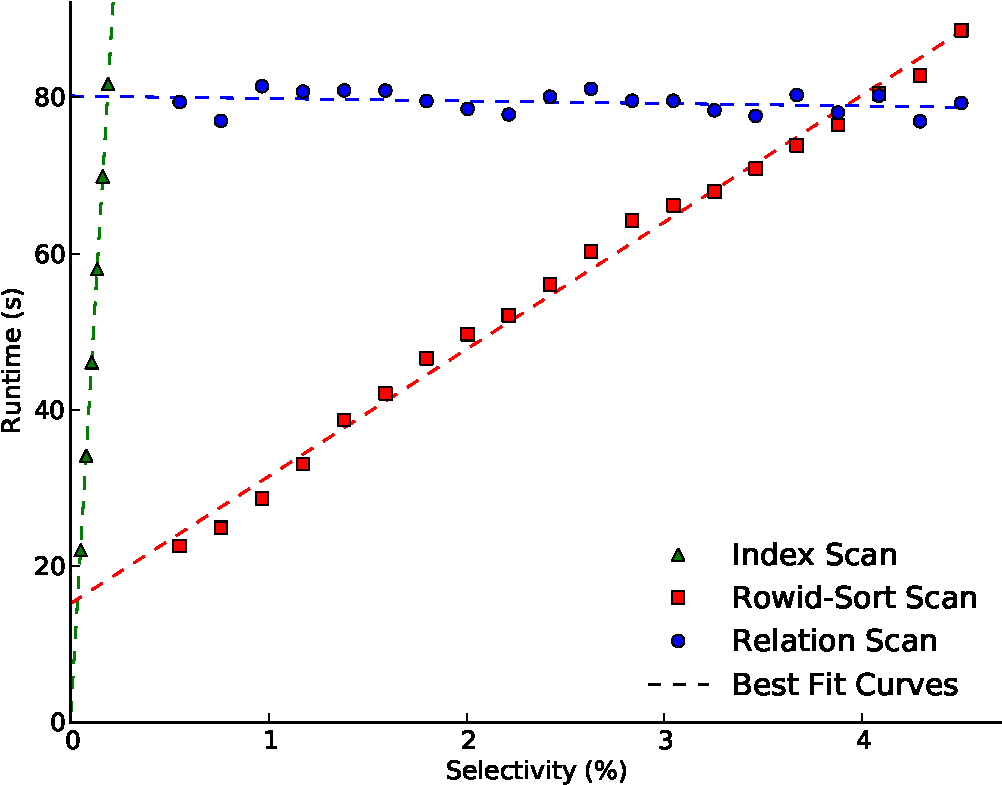
\includegraphics[width=5.0in]{FlashOpti/ScanDisk.pdf}
\caption{ \textbf{Scan operator performance on Disk.} Relation scan outperforms the alternatives at selectivities above 4\%, while index scan is optimal only for vanishingly small selectivities (e.g., single-tuple queries).  Best fit curves drawn for convenience.}
\label{fig:scan-disk}
%}
%\hspace{0.5in}
\end{figure*}
\begin{figure*}
\centering
%\subfigure[Flash SSD.]{
  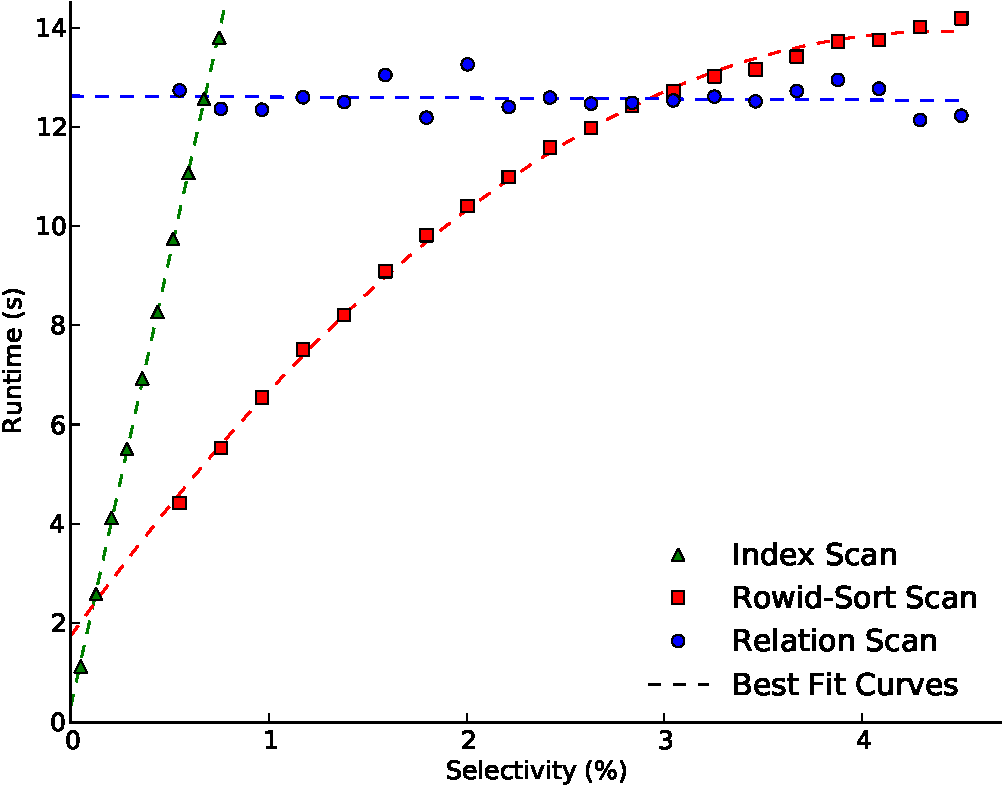
\includegraphics[width=5.0in]{FlashOpti/ScanFlash.pdf}
%}
\caption{ \textbf{Scan operator performance on Flash SSD.} Though both break-even points shift as our intuition suggests, the selectivities where the optimal decision differs between Disk and SSD are so narrow that the difference is inconsequential in practice.  Best fit curves drawn for convenience.}
\label{fig:scan-ssd}
\end{figure*}

I compare the measured performance of the different scan operators as a function of selectivity on SSD and disk.
The objective is to find the break-even points where the optimal scan operator shifts from index scan to rowid-sort scan and finally to relation scan on each device, and the performance impact in regions where this decision differs.
I issue queries for ranges of tuples using a uniformly distributed integer field on a table with 10 million rows, or roughly 2 GB. 
I use a pipelined aggregation function to ensure that no output table is materialized.

Figures~\ref{fig:scan-disk} and~\ref{fig:scan-ssd} report scan runtime on disk and Flash SSD, respectively.
The figures show the measured runtime of each scan (in seconds); lower is better. 
Recall from Section~\ref{sec:FlashOpti:Intro} that classic rules of thumb suggest that, on disk, the break-even point between index and relation scan should occur near 10\% selectivity, and intuition suggests an even higher break-even point for SSD.
Clearly, the conventional wisdom is flawed even for rotating disks; relation scan dominates above selectivities of just 4\% (the trends shown in the figure continue to the right).  
Indeed, the results indicate that even DB2's query optimizer is erroneously choosing to perform index scans at selectivities well below 0.55\% where both relation scan and rowid-sort scan still perform substantially better. 
In the intermediate range from about 0.1\% to 4\% selectivity the rowid-sort scan performs best.

However, the more important analysis is to compare the locations of the break-even points across SSD and disk.  
Both crossover points shift in the expected directions.
The slope of the index scan curve is considerably shallower, and the break-even with the relation scan shifts above 0.5\% selectivity.  
Furthermore, the range in which rowid-sort scan is optimal becomes narrower.
Nevertheless, the key take-away is that the range of selectivities for which the optimal scan \emph{differs} across SSD and Disk is vanishingly small.
Only a minute fraction of queries fit into this range, and those that make the incorrect decision (between disk and flash) see a small performance impact.
Hence, it is unnecessary for the optimizer to be SSD-aware to choose the correct scan operation.

Whereas these measurements demonstrate my main result, they do not explain why index scans fail to leverage the random access advantage of Flash.  
I turn to this question next. 

\textbf{Analytic Results.}
\begin{figure*}
\centering
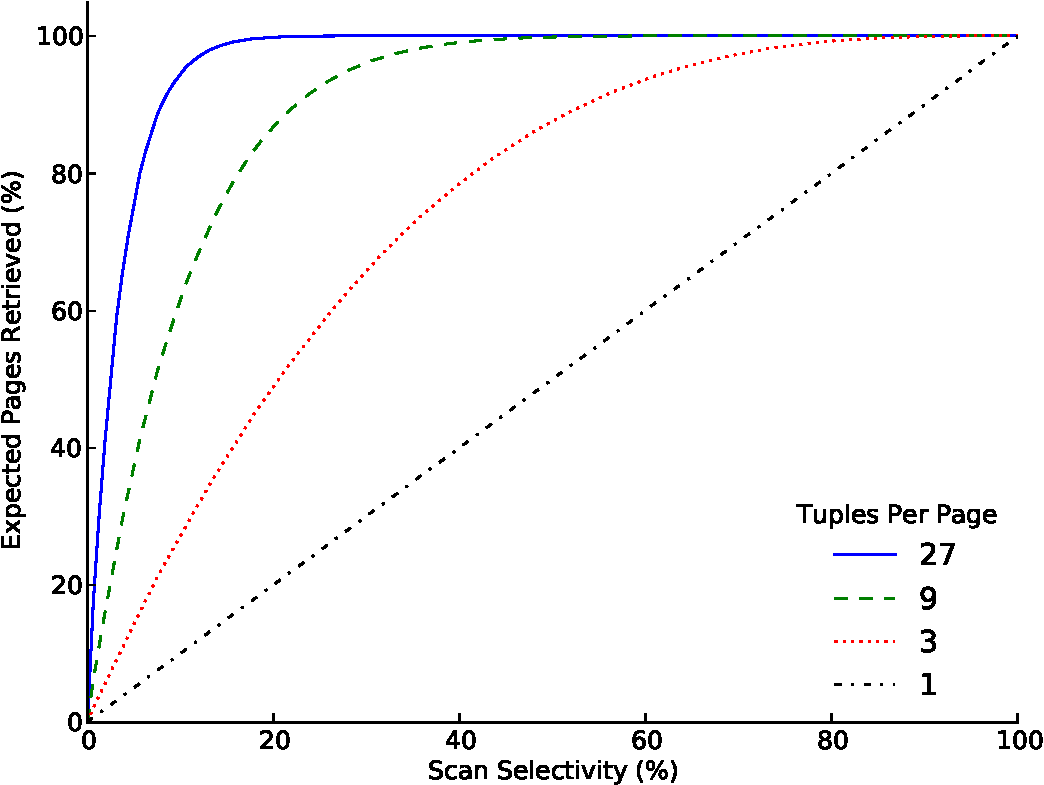
\includegraphics[width=5.0in]{FlashOpti/expectedPagesRet.pdf}
\caption{Index scans touch the majority of pages even at low selectivities.}
\label{figure::analyticScan}
\end{figure*}

The previous results show that index scans underperforms at selectivities far below what the classic 10\% rule of thumb suggests. 
The flaw in the conventional wisdom is that, when there are many tuples per page, the vast majority of \emph{pages} need to be retrieved even if only a few \emph{tuples} are accessed.
If the 10\% rule is applied to page- rather than tuple-selectivity, the guideline is more reasonable.
Yue \emph{et al.} provide an analytical formula for the expected number of pages retrieved given the size of the table, tuples per page, and selectivity \cite{Yue1975}, assuming tuples are randomly distributed among pages (a reasonable assumption given that each table can be clustered on only a single key).
Based on this formula, Figure~\ref{figure::analyticScan} shows the expected percentage of pages retrieved as a function of query selectivity and tuples per page.
When a page contains only a single tuple, clearly, the number of tuples and pages accessed are equal.
However, as the number of tuples per page increases, the expectation on the number of pages that must be retrieved quickly approaches 100\% even at small selectivities.
As a point of reference, given a 4kb page size and neglecting page headers, the Wisconsin Benchmark stores 19 tuples per page while TPC-H's Lineitem and Orders tables store 29 and 30 tuples per page, respectively.

The implication of this result is that, for typical tuple sizes, the vast majority of a relation must be read even if the selectivity is but a few percent.
Hence, with the exception of single-tuple lookups, there are few real-world scenarios where scan performance improves with better random access latency under conventional storage managers that access data in large blocks.
To benefit from low access latency, future devices will need to provide random access at tuple (rather than page) granularity.
Until we have such devices, relation and rowid-sort scans will dominate, with IO bandwidth primarily determining scan performance.

\section{Join Analysis}
\label{sec:FlashOpti:Joins}

We next study the variability in join performance across disk and Flash SSD.  
Again, the objective is to identify cases where the optimal join algorithm for disk consistently results in grossly sub-optimal performance on Flash SSD.
Such scenarios imply that it is important for the optimizer to be SSD aware.

DB2 implements nested loop, sort-merge, and hybrid hash join operators.  
However, DB2 does not support a block nested loop join; its nested loop join performs the join tuple-by-tuple instead of prefetching pages or other blocks, relying on indexes to provide high performance.
Hence, unless the join can be performed in memory, the nested loop grossly underperforms the other two algorithms for ad-hoc queries (those that do not use indexes) regardless of storage device and will not be selected by the query optimizer unless it is the only alternative (e.g., for inequality joins). 
I therefore restrict the investigation to a comparison of sort-merge and hybrid hash joins.

When a clustered index exists for a particular scan or join this index should almost always be used, regardless of the nature of the storage device.  
Hence, I do not include clustered indexes in my analysis.
Furthermore, I evaluate only ad hoc joins.
When indexes are available, the choice of whether or not to use the index is analogous to the choice of which scan operator to use for a simple select query, which is covered by the analysis of scans.

Because of the complexity of the interplay between available memory capacity and relation sizes for join optimization \cite{DBLP:journals/vldb/HaasCLS97}, I do not have a specific expectation that one join algorithm will universally outperform another on Flash SSD as opposed to disk.
Rather, I perform a cross-product of experiments over a wide spectrum of relation sizes and output projectivities using the Wisconsin Benchmark database.  
Haas's model demonstrates the importance of the relative sizes of input relations and main memory capacity on join performance; hence I explore a spectrum from joins that are only slightly larger than available memory (joining two 1.9GB tables) to those that are an order of magnitude larger (joining two 9.7GB tables).   
I vary projectivity, having discovered empirically that it significantly impacts the optimal join algorithm on disk, as it has a strong influence on partition size in hybrid hash joins.
I execute queries with two projectivities: approximately 5\% (achieved by selecting all the integer fields in the Wisconsin Benchmark schema), and approximately 25\% (selecting an integer field and one of the three strings in the schema).
In all experiments, I perform an equijoin on an integer field, and use an aggregation operator to avoid materializing the output.

\begin{figure*}
\centering
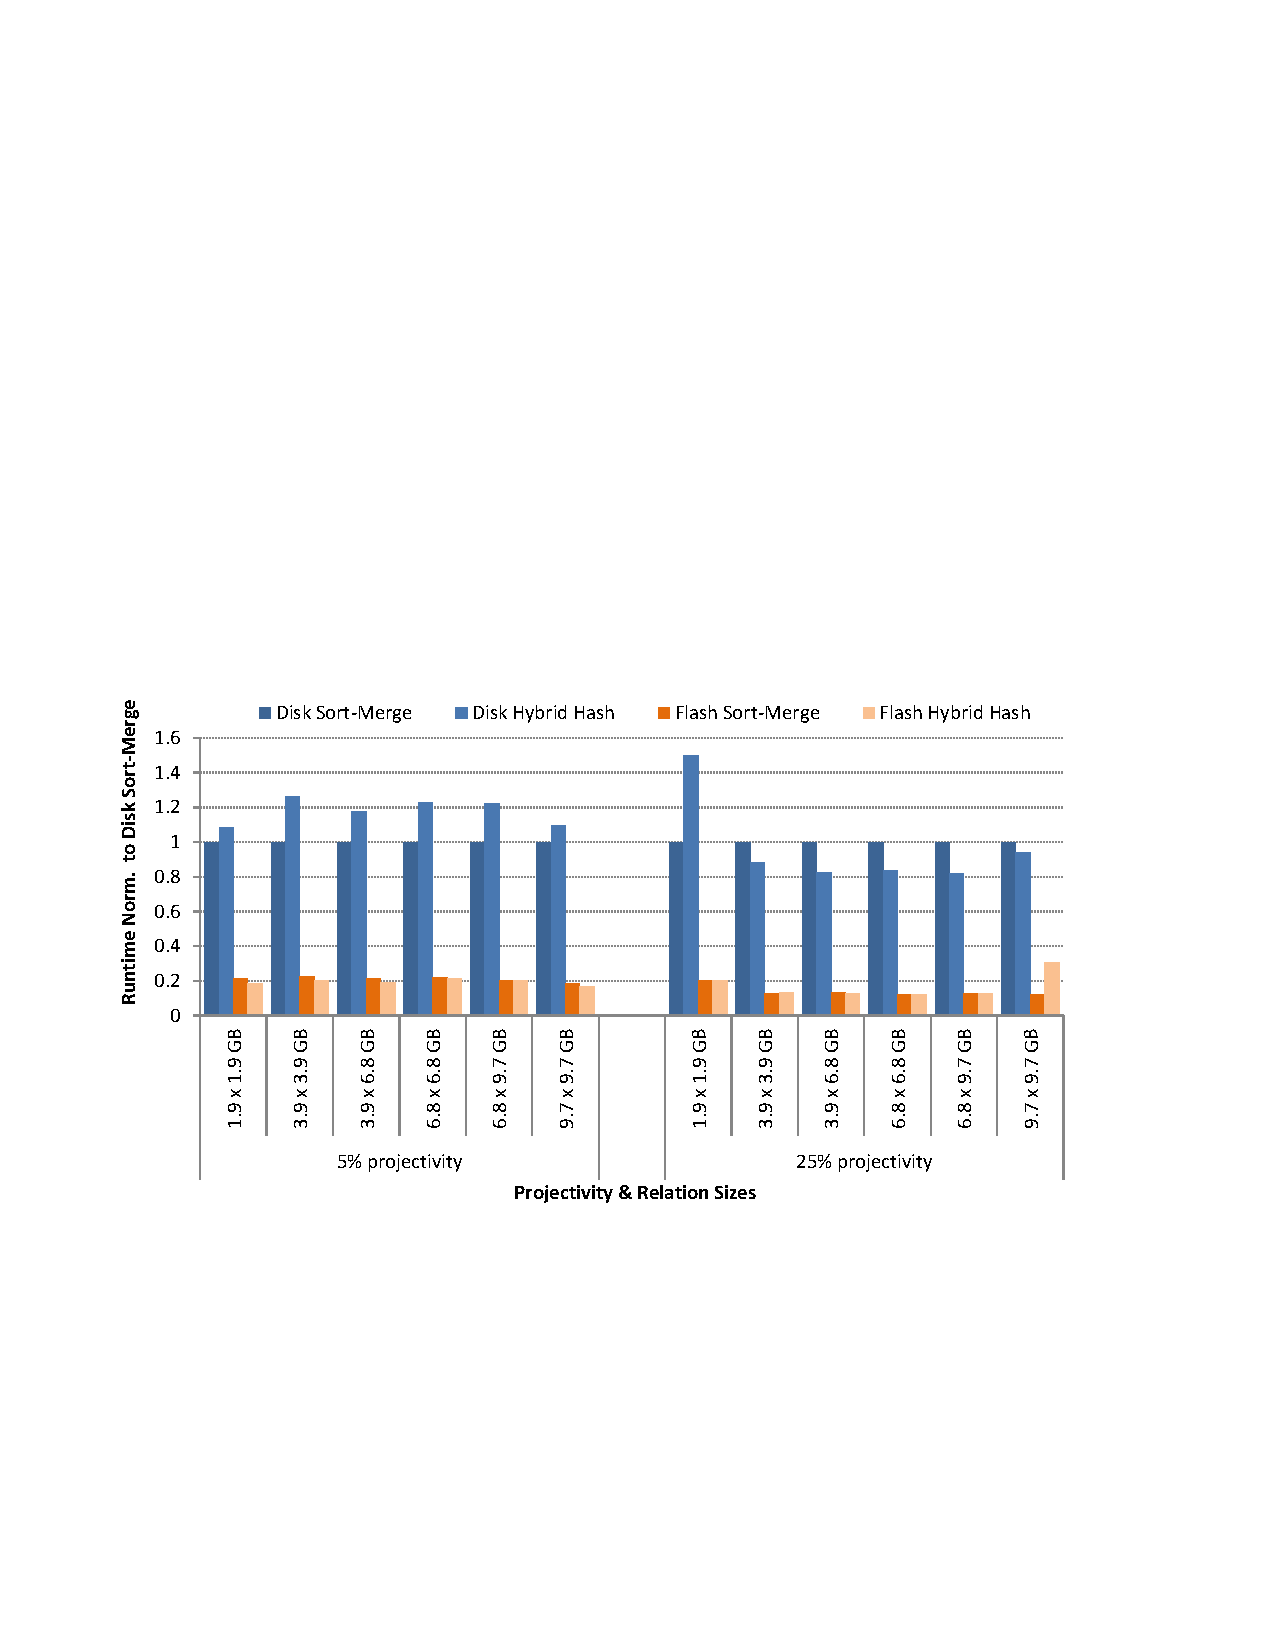
\includegraphics[width=6.0in]{FlashOpti/join.pdf}
\caption{\textbf{Join performance.}  Join runtimes on Flash SSD and Disk, normalized for each join to the runtime of sort-merge on disk.  Though there is significant variability in join algorithm performance on disk, performance variability on SSD is dwarfed by the  6\texttimes~performance advantage of moving data from disk to SSD.}
\label{figure::joins}
\end{figure*}


I report results in graphical form in Figure~\ref{figure::joins} and absolute runtimes in Table~\ref{table::joins}.
In Figure~\ref{figure::joins}, each group of bars shows the relative performance of sort-merge and hybrid hash joins on disk (darker bars) and Flash SSD (lighter bars), normalized to sort-merge performance on disk.
Lower bars indicate higher performance.
We provide the same data in tabular form to illustrate the runtime scaling trends with respect to relation size, which are obscured by the normalization in the graph.

Two critical results are immediately apparent from the graph.  
First, Flash SSDs typically outperform disk by 5\texttimes~to 6\texttimes~regardless of join algorithm, a margin that is substantially higher than the gap in sequential IO bandwidth, but far smaller than the gap in random IO bandwidth (see Table~\ref{table:DiskCharacteristics}).
Hence, though both join algorithms benefit from the improved random IO performance of SSDs, the benefit is muted compared to the 100\texttimes~device-level potential.
Second, we note that, whereas there is significant performance variability between the join algorithms on disk (typically over 20\%), with the exception of a single outlier, the variability is far smaller on Flash SSD (often less than 1\%).
From these results I conclude that although important on disk, the choice of sort-merge vs hybrid hash join on SSD leads to inconsequential performance differences relative to the drastic speedup of shifting data from disk to Flash.
Hence, there is no compelling reason to make the query optimizer SSD-aware; the choice it makes assuming the performance characteristics of a disk will yield near-optimal performance on SSD.

\begin{table*}
\centering
\begin{tabular}{c@{\hspace{12pt}}c@{\hspace{12pt}}c@{\hspace{12pt}}c@{\hspace{1pt}}c@{\hspace{12pt}}c@{\hspace{12pt}}c}
%\begin{tabular}{c  c | c | c | c | c}
  \toprule
	\multirow{2}{*}{Projectivity} 		      & \multirow{2}{*}{Table Sizes} & \multicolumn{2}{c}{Disk}    & &  \multicolumn{2}{c}{Flash SSD}  \\ 
\cmidrule{3-4} \cmidrule{6-7}
	 &  & Sort-merge & Hybrid hash     & &  Sort-merge & Hybrid hash  \\ 
   \midrule
5\%	& 1.9 x 1.9 GB	& 187 	& 202	& & 40		& 34	\\
	& 3.9 x 3.9 GB	& 358	& 451	& & 80		& 72	\\
	& 3.9 x 6.8 GB	& 487	& 574	& & 103	& 93	\\
	& 6.8 x 6.8 GB	& 649	& 795	& & 142	& 140\\
	& 6.8 x 9.7 GB	& 816	& 997	& & 166	& 166\\
	& 9.7 x 9.7 GB	& 1084	& 1189	& & 202	& 183\\
  \midrule
25\% & 1.9 x 1.9 GB	& 236	& 355	& & 48		& 48	\\
	& 3.9 x 3.9 GB	& 751	& 662	& & 97		& 101\\
	& 3.9 x 6.8 GB	& 947	& 781	& & 125	& 122\\
	& 6.8 x 6.8 GB	& 1415	& 1182	& & 174	& 173\\
	& 6.8 x 9.7 GB	& 1581	& 1298	& & 199	& 199\\
	& 9.7 x 9.7 GB	& 2081	& 1955	& & 250	& 634\\
  \bottomrule
\end{tabular}
\caption{\textbf{Absolute join performance.}  Join runtimes in seconds.  Variability in join runtimes is far lower on Flash SSD than on Disk.}
\label{table::joins}
\end{table*}



I highlight two notable outliers in our results.
On disk, the best join algorithm is strongly correlated to query projectivity with the exception of the 1.9GB~\texttimes~1.9GB join at 25\% projectivity.
Because the required hash table size for this join is close to the main memory capacity, I believe that this performance aberration arises due to DB2 selecting poor partition sizes for the join.
Second, on Flash, I observe a large performance difference (over 2\texttimes) between sort-merge and hybrid hash join for our largest test case, a 9.7GB~\texttimes~9.7GB join at 25\% projectivity.
For this query, we observe a long cpu-bound period with negligible IO at the end of the hybrid hash join that does not occur for any of the other hash joins.
Hence, I believe that this performance aberration is unrelated to the type of storage device, and may have arisen due to the methods employed to coax the optimizer to choose this join algorithm.
In any event, neither of these outliers outweigh the broader conclusion that there is no particular need for the query optimizer to be SSD aware.

\section{Related Work}
\label{sec:FlashOpti:RelatedWork}
Previous work studying the applicability of Flash memory in DBMS applications has focused on characterizing Flash, benchmarking specific database operations on Flash, and designing new layouts, data structures, and algorithms for use with Flash.

Both Bouganim \emph{et al.} and Chen \emph{et al.} benchmark the performance of Flash for various IO access patterns \cite{Bouganim09uflip:understanding, Chen2009}.
Bouganim introduces the uFLIP micro-benchmarks and tests their performance on several devices.
Chen introduces another set of micro-benchmarks, concluding that poor random write performance poses a significant barrier to replacing conventional hard disks with Flash SSDs.
While these micro-benchmarks are instructive for understanding database performance, I focus specifically on the performance of existing scan and join operators on SSD and disk.
Others have also benchmarked Flash's performance within the context of DBMS systems.
Lee \emph{et al.} investigate the performance of specific database operations on Flash, including multiversion concurrency control (MVCC), external sort, and hashes \cite{Lee2008}.
Similar to my study, Do \emph{et al.} benchmark ad hoc joins, testing the effects of buffer pool size and page size on performance for both disk and Flash \cite{Do2009}.
Although related to this study, neither of these works look at the specific performance differences between disk and Flash for scans and joins and how this might impact query optimization.

Whereas the above works (and this study) focus on measuring the performance of existing databases and devices, others look ahead to redesign DBMS systems in light of the characteristics of Flash.
Yin \emph{et al.} and Li \emph{et al.} present new index structures, focusing on maintaining performance while using sequential writes to update the index \cite{Yin2009, Li2009}.
Baumann \emph{et al.} investigate Flash's performance alongside a hybrid row-column store referred to as ``Grouping" \cite{Baumann2010}.
Similarly, Tsirogiannis \emph{et al.} use a column store motivated by the PAX layout to create faster scans and joins \cite{Tsirogiannis2009}.

Interestingly, my findings contradict recommendations of these last two studies.
Baumann concludes that SSDs shift optimal query execution towards index-based query plans.
The study bases this conclusion on the observation that asynchronous random reads on Flash are nearly as fast as sequential reads.
Indeed, the arguments made by Baumann are a key component of the intuition laid out in Section~\ref{sec:FlashOpti:Intro} that led me to expect a need for SSD-aware query optimization.
However, the conclusion neglects the observations discussed in Section~\ref{sec:FlashOpti:Scans} demonstrating that queries selecting more than a handful of tuples will likely retrieve the majority of pages in a relation, and thus gain no advantage from fast random IO.
Tsirogiannis introduces a join algorithm that retrieves only the join columns, joins these values, and then retrieves projected rows via a temporary index.
By our previous argument, scanning for projected data should retrieve the majority of data pages, preferring a relation scan, and thus provide comparable advantage on disk and SSD.
I leave a comparative evaluation of their FlashJoin algorithm on SSD and disk to future work.

\section{Conclusion}
\label{sec:FlashOpti:Conclusion}
Flash-based solid state disks provide an exciting new high-performance alternative to disk drives for database applications.
My investigation of SSD-aware query optimization was motivated by a hope that the drastically improved random IO performance on SSDs would result in a large shift in optimal query plans relative to existing optimizations.
At a minimum, I expected that constants capturing relative IO costs in the optimizer would require update.
This chapter presented evidence that refutes this expectation, instead showing that an SSD-oblivious query optimizer is unlikely to make significant errors in choosing access paths or join algorithms.
Specifically, I demonstrate both empirically and analytically that the range of selectivities for which a scan operation can benefit from SSDs' fast random reads is so narrow that it is inconsequential in practice.
Moreover, measurements of alternative join algorithms reveal that their performance variability is far smaller on SSDs and is dwarfed by the 5\texttimes~to 6\texttimes~performance boost of shifting data to SSD. 
Overall, I conclude that the small and inconsistent performance gains available by making query optimizers SSD-aware are not worth the effort.
